\section{Architecture}
\label{sec:arch}

\begin{figure}[t]
\centering
   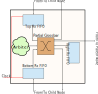
\includegraphics[height=0.5\columnwidth]{Figures/switch1.pdf}
   \caption{Architecture of the proposed FPGA based neural network evaluation platform}
   \label{fig:switchArch}
\end{figure}


\begin{figure}[t]
\centering
   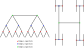
\includegraphics[height=0.5\columnwidth]{Figures/HNoC.pdf}
   \caption{Architecture of the proposed FPGA based neural network evaluation platform}
   \label{fig:switchArch}
\end{figure}

\subsection{Switch}
The architecture of the proposed NoC type-1 switch is as shown in Fig.~\ref{fig:switchArch}.
Each receive and transmit interfaces of the switch for the child nodes are connects to an asynchronous FIFO.
The interface to the parent node contains a single synchronous FIFO for the receive interface.
Thus each switch contains 5 FIFOs.
The depth of the FIFOs are kept very low (16) to reduce the resource utilization.
The asynchronous FIFOs receive data from the downstream ports on Clock 1 signal
The received packets are routed to the appropriate output ports by an arbitrator through a cross-bar switch.
The transmit side of the FIFO as well as the arbitrator and the cross bar works on Clock 2 signal, whose frequency will be much higher than that of Clock 1 (ideally twice as much as Clock 1).

The arbitrator internally uses flit-level round-robin arbitration scheme to select the input port when more than one port requests for the same output port.
If a single port is requesting for a particular out, it is given the access until all the flits are sent out.
